% FID values for run2, run4 and run5
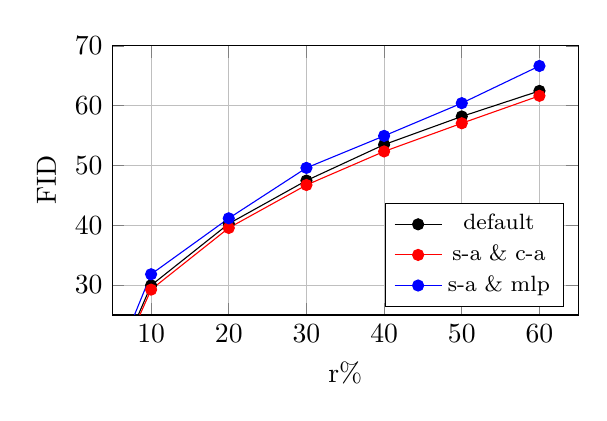
\begin{tikzpicture}
\begin{axis}[
    title={},
    height=5cm,
    width=7.5cm,
    xlabel={r\%},
    ylabel={FID},
    xmin=5, xmax=65,
    ymin=25, ymax=70,
    xtick={10,20,30,40,50,60},
    ytick={30,40,50,60,70},
    legend pos=south east,
    xmajorgrids=true,
    ymajorgrids=true,
    legend style={font=\footnotesize}
]

\addplot[
    color=black,
    mark=*
    ]
    coordinates {
    (0,0)(10,29.95)(20,40.26)(30,47.47)(40,53.48)(50,58.19)(60,62.46)
    };
    
\addplot[
    color=red,
    mark=*
    ]
    coordinates {
    (0,0)(10,29.24)(20,39.55)(30,46.73)(40,52.34)(50,57.05)(60,61.64)
    };

\addplot[
    color=blue,
    mark=*
    ]
    coordinates {
    (0,0)(10,31.81)(20,41.16)(30,49.59)(40,54.94)(50,60.41)(60,66.63)
    };
    
\legend{default, s-a \& c-a, s-a \& mlp}
    
\end{axis}
\end{tikzpicture}